%%%  ___       _
%%% |_ _|_ __ | |_ _ __ ___
%%%  | || '_ \| __| '__/ _ \
%%%  | || | | | |_| | | (_) |
%%% |___|_| |_|\__|_|  \___/
%%%
%%% TCC de Bianca Miyabe Santos Freitas
%%% Licenciatura em Física - UFSCar, Sorocaba
%%%
\chapter{Introdução}

Nas últimas décadas a humanidade passou por um intenso e revolucionário processo de inovações e renovações tecnológicas envolvendo o dispositivo que conhecemos por computador. Basta recordar que o tamanho de um smartphone moderno é muito menor do que a primeira unidade de computador eletrônico criado, o ENIAC, que ocupava um espaço de \SI{180}{\square\meter} \cite{eniac}.

Nesse processo evolutivo do computador podemos destacar que a miniaturização dos processadores resultou no aumento da sua capacidade de processamento de informação e estes foram essenciais para a popularização dos dispositivos e ainda, para o aumento da sua velocidade operacional. Diante dessa constante mudança, em 1965 foi estabelecido por Gordon E. Moore um limite de processamento devido ao número de transistores\footnote{O transistor é um componente eletrônico desenvolvido por John Bardeen, William Shockley e Walter Brattain em meados de 1947. O dispositivo passou por diversos aperfeiçoamentos desde então e sua principal função consiste em amplificar ou interromper sinais elétricos. Nos computadores, são os responsáveis por indicar a presença ou ausência do sinal elétrico, sendo possível a interpretação da informação nos dispositivos de processamento \cite{transistor}.} necessários comprimidos em um pequeno espaço versus sua dissipação de calor, o que corrompe a informação. Esse limite recebeu o nome de ``Lei de Moore''. Nela, \textcite{moore} estimou que o número de transistores de um computador dobraria a cada dois anos sem que seu valor fosse alterado. Esse limite foi brevemente superado por novas tecnologias de materiais\footnote{A empresa IBM, produziu em 2014 um nanochip de silício de \SI{7}{\nano\meter} e em 2015 anunciou a produção de chips de processamento com nanotubos de carbono de tamanho \SI{1.8}{\nano\meter} \cite{chipibm}.}, deixando evidente, entretanto, a necessidade de expandir a capacidade de processamento dos sistemas atuais, visto que a tendência de crescimento na quantidade de informação processada é cada vez maior.

Diante do limite físico para o tamanho dos processadores e do crescimento do volume de informação a ser processado, uma possível solução foi proposta pelo físico Richard Feynman em 1981. Feynman, na tentativa de compreender a simulação de sistemas físicos para seus estudos, propõe que se sistemas físicos são regidos pela física quântica, sua simulação deve ser feita por um dispositivo que corresponda a mesma natureza \cite{caldeira}.

Nesse período temos portanto a junção de três importantes áreas de estudo: a computação, a informação e a física quântica. Esta união visava superar os limites da computação até então, em relação à velocidade de processamento e volume de armazenamento de informação, dando início aos estudos da chamada \textit{Computação Quântica}. A computação quântica é um campo emergente cujo objetivo é desenvolver computação com base nos princípios da mecânica quântica que, conforme veremos na Seção~\ref{sec:Mecanicaquantica}, é a teoria da Física que descreve o comportamento dos átomos, íons e partículas subatômicas. As partículas quânticas podem existir em múltiplos estados ao mesmo tempo e essa característica única permite que os computadores quânticos manipulem simultaneamente muitos estados de dados, o que não é possível com computadores convencionais, permitindo aos computadores quânticos processar muito mais informação, de forma mais rápida e eficiente do que os computadores convencionais, que utilizam a arquitetura de dados clássica, ou seja, informação clássica \cite{CompInfoQuantica}.

Segundo \textcite{conceitoinformação}, o conceito de informação possui seu significado cotidianamente atribuído como \textit{conhecimento comunicado}. Nesse sentido, a informação já existia nas pinturas rupestres há cerca de \num{45.5} mil anos atrás, nas quais estão registradas uma série de imagens no intuito de comunicar, seja um evento ou ainda uma quantidade. Apesar do conceito de informação aparecer desde os primórdios do estabelecimento da humanidade, é apenas na década de 1940 que esta passa a ser objeto de estudo com os trabalhos de Claude Elwood Shannon (1916--2001), que desenvolve uma teoria matemática para a informação \cite{CiênciaTransiçãoSeculosa}.

O objetivo principal da Teoria da Comunicação de Shannon ou \textit{Teoria Matemática da Comunicação} (TMC), era sistematizar o conhecimento acumulado até então acerca da eficiência em sistemas de comunicação, ou seja, de como a informação é transmitida. A teoria descreve o funcionamento lógico-matemático de um destes sistemas, composto por um gerador de informação, um meio de transmissão e um receptor, conforme ilustra a Figura~\ref{comunicshannon} \cite{MTC}.

\begin{figure}[ht!]
  \centering
  \caption{Esquema geral de um sistema de comunicação com a Fonte de Informação criando uma Mensagem a ser transmitida pelo Transmissor que a transforma em um Sinal. Na transmissão pode haver uma Fonte de Ruído. O sinal é recebido pelo Receptor e finalmente a mensagem chega ao seu Destino.}\label{comunicshannon}
  % 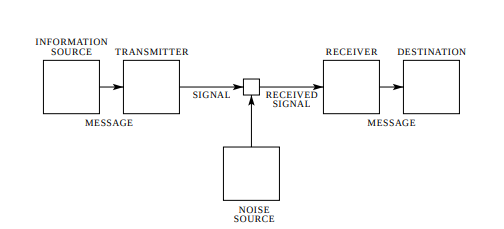
\includegraphics[width=0.65\textwidth]{comunicadorshannon.png}
  \begin{tikzpicture}
    \matrix (A) [matrix of nodes,
    column sep=25pt,
    row sep=30pt,
    nodes={minimum size=35pt}]
    {
      \node[label={[labelst]above:Fonte de\\informação},blocoq] (fonte) {}; &
      \node[label={[labelst]above:Transmissor},blocoq] (trans) {}; &
      \node[minimum size=10pt,blocoq] (conn) {}; &
      \node[label={[labelst]above:Receptor},blocoq] (rec) {}; &
      \node[label={[labelst]above:Destino},blocoq] (dest) {}; \\
      & & \node[label={[labelst]below:Fonte de \\ruído},blocoq] (ruido) {}; \\
    };
    \draw[conecta] (fonte) -- node[pos=0.5,below,labelst,yshift=-20pt] {Mensagem} (trans);
    \draw[conecta] (trans) -- node[pos=0.5,below,labelst] {Sinal} (conn);
    \draw[conecta] (conn) --  node[pos=0.5,below,labelst] {Sinal\\recebido} (rec);
    \draw[conecta] (rec) -- node[pos=0.5,below,labelst,yshift=-20pt] {Mensagem} (dest);
    \draw[conecta] (ruido) -- (conn);
  \end{tikzpicture}
  \fonte{Adaptado de \textcite[p. 380]{MTC}.}
\end{figure}

De acordo com  a TMC, um \textit{gerador de informação} é um objeto capaz de produzir um conjunto $X$ de $n$ eventos com probabilidade de ocorrência $P(X)$, enquanto um \textit{receptor} possui um conjunto $Y$, também com $n$ eventos, com probabilidades associadas $P(Y)$. Durante a transmissão é possível que parte da informação seja perdida devido a ocorrência de ruídos, o que resulta diretamente na modificação dos valores de probabilidade dos elementos recebidos do conjunto $Y$. Reconhecendo portanto os elementos de $X$ e suas probabilidades associadas, espera-se que uma mensagem bem transmitida, ou seja, sem interferência de ruídos, seja aquela cujas probabilidades dos elementos do conjunto $Y$ sejam as mesmas dos elementos do conjunto $X$. Assim, se essas probabilidades forem distintas, podemos concluir que houve perda de informação na transmissão \cite{mathematical}.

De maneira geral, a informação é quantificada de acordo com os recursos físicos necessários para que ela seja representada, ou seja, na capacidade de armazenamento, comunicação e representação de um conjunto $X$ de possíveis informações. Em um computador clássico, por exemplo, armazenamos informações através das unidades binárias chamadas \textit{bits}\footnote{Nome proposto, segundo o artigo original de Shannon por J.W. Turkey \cite{MTC}.}. Dessa forma, os bits são a menor unidade de armazenamento de informação em um computador de arquitetura clássica, podendo representar o estado 1 ou o estado 0 \cite{MTC}.

A combinação desses bits faz com que uma mensagem possa ser armazenada, processada ou transmitida em um computador clássico. Nesse sentido, quão maior, ou ainda, quão mais complexa for a mensagem a se operar, mais bits serão necessários e consequentemente mais recursos físicos para a representação destes.

A descrição da arquitetura de um computador quântico esbarra no mesmo princípio daquela de um computador clássico, ou seja, em sua unidade fundamental de armazenamento de informação. De maneira análoga ao computador clássico, que utiliza como unidade de informação o bit, o computador quântico utilizará o \textit{qubit} (ou q-bit, ou ainda, quantum bit).

Um qubit, ou bit quântico, pode ser produzido de maneiras distintas\footnote{Qubits podem ser fisicamente criados utilizando, por exemplo, spins de átomos presos em uma armadilha. Essa armadilha pode ser do tipo óptica ou até mesmo magnética. É possível também polarizar fótons para sua obtenção. A determinação do método é definida principalmente pelo mecanismo que melhor conseguir isolar o qubit, já que este é facilmente influenciado pelo ambiente externo \cite{materialdidaticomecquantica}.}, porém nosso foco de estudo está nas suas propriedades. Um qubit é uma unidade com propriedades quânticas que atua sob o regime de superposição de estados. Isso significa que ele consegue armazenar simultaneamente mais de um estado de informação, diferente do bit clássico que armazena apenas um dos estados por vez. Decorre desta propriedade a maior capacidade de operar a informação em comparação aos mecanismos clássicos segundo apresentado na Tabela~\ref{tabelabit}.

\begin{table}[ht]
  \centering
  \caption{Comparação entre a quantidade de bits clássicos e quânticos necessários para se operar uma informação.}\label{tabelabit}
  \begin{tabular}{ccc}
    \toprule
    \thead{Quantidade \\ de bytes \\ (informação)} & \thead{Quantidade \\ de bits clássicos} & \thead{Quantidade \\ de qubits} \\
    \midrule
    1         & 8            & 3  \\
    \num{e6}  & \num{8.3e6}  & 23 \\
    \num{e12} & \num{8.8e12} & 43 \\
    \bottomrule
  \end{tabular}
  \fonte{Elaborada pelo autor.}
\end{table}

De modo a generalizar a comparação entre bits classicos e quânticos, podemos estabelecer a relação:
\begin{equation} \label{bitvsqubit}
n\, \text{qubits} = 2^{n}\,\text{bits}.
\end{equation}

Portanto, podemos concluir que menos qubits são necessários para operar a informação, em comparação ao bit clássico, o que está diretamente relacionado com a velocidade e com a capacidade de realização deste.

Segundo \textcite{CompInfoQuantica} e \textcite{dwave}, a devida construção de um computador de arquitetura quântica foi precedida pelos eventos descritos a seguir:

\begin{description}
  \item[1985] David Deustch propõe matematicamente o primeiro computador quântico universal;
  \item[1994] Peter Shor cria o primeiro programa essencialmente quântico, ou seja, ele não poderia ser executado em um computador clássico. Este programa, conhecido como Algoritmo de Shor, reduziria o tempo de fatoração de números grandes de possíveis meses para apenas segundos caso fosse utilizado em um computador real de arquitetura quântica;
  \item[1999] O MIT apresenta o primeiro protótipo de um computador quântico real;
  \item[2007] A empresa D-Wave apresenta o primeiro computador essencialmente quântico.
\end{description}

Apesar de na atualidade processadores quânticos existirem e operarem\footnote{Atualmente a IBM possuí um processador que opera com 433 qubits simultâneos, o \textit{Osprey}, anunciado em novembro de 2022 \cite{osprey}.}, ainda estamos distantes da efetiva implementação comercial de um computador quântico. Podemos utilizar de exemplo, o fato de que apesar de possuirmos um análogo para a TMC de Shannon em um computador quântico\footnote{Em 1995, Benjamin Schumacher propõe com êxito um análogo quântico para o TMC \cite{benschu}.}, ainda não temos um análogo quântico para um sistema submetido a ruídos na transmissão\footnote{Contudo, foi desenvolvida a teoria de correção de erros quânticos que permite que computadores quânticos possam operar na presença de ruídos e que a informação quântica seja transmitida de maneira confiável \cite{chuang}}\cite{chuang}.

Portanto, o estudo de simulações de sistemas de informação quânticos se faz necessário para aperfeiçoamento desses mecanismos e ainda para o desenvolvimento da própria Física, visto que o avanço da compreensão da utilização da mecânica quântica atrelado ao conceito de informação, possibilita a compreensão da natureza de maneira cada vez mais complexa, sem a necessidade de aproximações e simplificações \cite{chuang}.

Devido aos recursos de simulação, podemos utilizar um computador de arquitetura clássica para simular tanto um qubit quanto os circuitos lógicos necessários para a realização de operações com a informação quântica, a título do estudo, por exemplo, dos efeitos de ruídos na transmissão da informação quântica conforme propomos nesse trabalho. Nesse sentido, os próximos capítulos irão introduzir conceitos sobre informação quântica e mecânica quântica para a compreensão do desenvolvimento do trabalho.
